\section{Erläuterung Fallstudie}
Nachdem die theoretischen Grundlagen nun erläutert worden sind, wird mit der Fallstudie begonnen. Für die Fallstudie soll ein vereinfachtes \ac{CRM-System} entwickelt und bereitgestellt werden. Ein \ac{CRM-System} ist eine Software für das Kundenbeziehungsmanagement. In diesem Kapitel werden die Anforderungen an das \ac{CRM-System} beschrieben.

\subsection{Anwendungseinsatz}
Das CRM-System soll für das \ac{B2C} Umfeld entwickelt werden. Die Kernfunktionalität des zu erstellenden CRM-Systems ist das Anlegen, Anzeigen, Bearbeiten und Löschen von Kontakten, Interaktionen und Verkaufschancen. Die Software soll mit einer Microservice-Architektur umgesetzt werden und containerisiert mit Kubernetes bereitgestellt werden. Das System soll über eine grafische Benutzeroberfläche mit einem Webbrowser bedienbar sein.

\subsection{Anwendungsfunktionen}
Das CRM-System soll die folgenden primären Funktionen implementieren:
\begin{itemize}
\item Kontakte sollen mit Namen, Geburtsdatum, Geschlecht, Telefonnummer, E-Mail-Adresse und Adresse angelegt, angezeigt, geändert und gelöscht werden können
\item Interaktionen mit einem Kontakt sollen mit Art der Interaktion, Datum, Uhrzeit, Notizen und dem zugehörigen Kontakt angelegt, angezeigt, geändert und gelöscht werden können
\item Mögliche Verkaufschancen sollen mit Status, voraussichtlichem Abschlussdatum, Verkaufswert, Rabatt, Budget des Kunden, Notizen und dem zugehörigen Kontakt angelegt, angezeigt, geändert und gelöscht werden können
\item Benutzung aller Funktionen über eine grafische Benutzeroberfläche mit einem Webbrowser
\item Benutzung aller Funktionen über eine REST-API
\end{itemize} 

Die Zugriffskontrolle und Benutzersicherheit wird bei der Anwendung nicht beachtet.

\section{Entwurf der Microservices}

Als Erstes wird die Architektur der Microservices festgelegt. Bei der Architektur kann zwischen Makro-Architektur und Mikro-Architektur unterschieden werden. Die Makro-Architektur befasst sich mit dem Microservice-System als Ganzes. In der Mikro-Architektur geht es um den Aufbau der einzelnen Microservices.

\subsection{Makro-Architektur}

Die Makro-Architektur befasst sich mit dem Enwurf des Gesamtsystems. Die Aufteilung der Funktionalitäten auf die Microservices und die Kommunikationstechnologien für die Integration der einzelnen Microservices ist hier von Interesse. Wie genau die einzelnen Microservices umgesetzt werden und welcher Technologie-Stack verwendet wird, ist für das Gesamtsystem nicht relevant. 

\begin{figure}[H] 
    \centering
    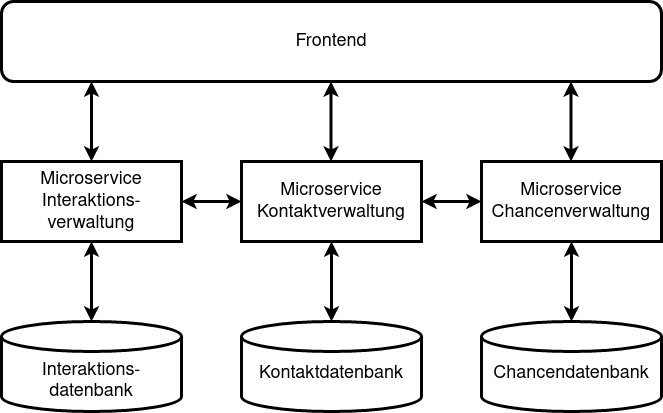
\includegraphics[width=0.71\textwidth]{figures/CRMEntwurf.png}
    \caption{Entwurf des CRM-Systems}
\end{figure}

\subsection{Micro-Architektur}

Die Mikro-Architektur befasst sich mit der Architektur eines einzelnen Microservice. Für das Gesamtsystem ist die Architektur eines einzelnen Microservice nicht von Bedeutung. Aus diesem Grund besitzt man eine große Freiheit bei der Auswahl. Es sollte die Architektur, welche am Simpelsten alle Anforderungen bietet. Der ausgewählte Technologie-Stack schränkt natürlich die möglichen Architekturen auch weiter ein.

Unser System besteht aus drei Microservices und einem Frontend. Das Frontend dient lediglich zur Visualisierung und Verbindung aller Funktionen der drei Microservices. Da eine Frontend 

Für die Architektur der Microservices wird eine hexagonale Architektur verwendet. Eine Hexagonale Architektur bietet sich 


\section{Implementierung}


\subsection{Microservices}

\subsection{Frontend}

Das Frontend. Das Frontend soll später auch mit Kubernetes bereitgestellt werden, es wird aber nicht als Microservices angesehen.

\section{Bereitstellung mit Kubernetes}

\subsection{Containerisierung}

\subsection{Bereitstellung}

\subsection{Skalierung}

\subsection{Lastverteilung}

